% Phase 2: exact oracle, baselines, MCMC sampler

\section{Exact oracle, convex/combinatorial baselines, MCMC sampler}\label{sec:oracle}

\subsection{Problem formulation}\label{ssec:formulation}

Fix a cardinality $k$ and risk-aversion $\gamma>0$. The cardinality-constrained
\emph{equal-weight Markowitz objective} is
\begin{equation}\label{eq:Jdef}
  J(\sigma) \;:=\; \frac{1}{k}\, \hat\mu^\top\sigma \;-\; \frac{\gamma}{2 k^2}\,\sigma^\top
  \hat\Sigma\sigma, \qquad \sigma\in\Omega_{n,k},
\end{equation}
where $\Omega_{n,k} := \{\sigma\in\{0,1\}^n : \sum_i\sigma_i = k\}$ is the cardinality-$k$
slice. We use $\gamma=10$ throughout. Equation~\eqref{eq:Jdef} arises from
mean-variance optimisation under the constraint $w_i = \sigma_i / k$ (equal weights on
the chosen support); allowing continuous weights modifies only constants in the analysis
and does not change the combinatorial difficulty. The decision problem we attack is
\begin{equation}\label{eq:problem}
  \sigma^\star \;:=\; \arg\max_{\sigma\in\Omega_{n,k}} J(\sigma).
\end{equation}

\subsection{Brute-force oracle}\label{ssec:oracle}

For sufficiently small $(n,k)$ the problem is solved exactly by enumerating all
$\binom{n}{k}$ subsets. Vectorised numpy with chunked indexing runs the
$(n,k)=(50,5)$ instance ($\binom{50}{5}\approx 2.1\times 10^6$ subsets) in $0.75$\,s
on a single core. We treat the resulting $\sigma^\star$ as the ground-truth oracle in
all subsequent benchmarks. Beyond $\binom{n}{k}\sim 10^7$ enumeration becomes infeasible
in wall-clock time; for such cells we use the matched-density brute-force regime
$(n,k)=(30,6)$ in Phase~3b and rely on near-oracle simulated annealing as a sanity check.

\subsection{Baselines}\label{sec:lasso}

We benchmark four polynomial-time algorithms taught in standard portfolio-optimisation
practice and connected to course concepts:
\begin{enumerate}\itemsep=2pt
  \item \emph{Top-eigenvector projection.} Output $S = \arg\mathrm{topk}_i\, |v_1(\hat\Sigma)_i|$
        where $v_1(\hat\Sigma)$ is the leading eigenvector of $\hat\Sigma$ (the spectral
        method, equivalent to PCA-based stock picking).
  \item \emph{Greedy forward selection.} Start from $S=\emptyset$ and at each step add the
        single asset that maximises $J(S\cup\{j\})$ until $|S|=k$.
  \item \emph{LASSO-Markowitz.} Solve the unconstrained $\ell_1$-regularised mean-variance
        program
        \[
          \hat w_\lambda \;=\; \arg\min_{w\in\mathbb R^n}\; \tfrac{\gamma}{2}\, w^\top\hat\Sigma w - \hat\mu^\top w
          + \lambda\,\|w\|_1,
        \]
        bisecting $\lambda$ until $|\,\mathrm{supp}(\hat w_\lambda)\,| = k$ and outputting
        the top-$k$ indices by $|\hat w_\lambda|$. CVXPY/CLARABEL-backed.
  \item \emph{Single-shot simulated annealing.} Constrained Metropolis on the slice
        $\Omega_{n,k}$ with swap proposals and a geometric cooling schedule
        $\beta_t = \beta_0 r^t$, $\beta_0=10^2,\beta_T=5\!\times\!10^4$; run for $10{,}000$
        sweeps from a random initial state and track the running best $J$.
\end{enumerate}

\subsection{Quantitative comparison on the oracle grid}\label{ssec:p2a-results}

Five random asset draws per cell, $\gamma=10$, train block. Mean optimality gap to the oracle
(in basis points, $1$\,bp = $10^{-4}$ in daily-return units of $J$) and mean wall-clock per call:

\begin{center}\small
\begin{tabular}{c|cc|cc|cc|cc}
$(n,k)$ & top-eig & ms & greedy & ms & LASSO & ms & sim-anneal & ms \\\hline
(20,5) & $14.0$ & $0.1$  & $0.05$ & $0.5$ & $6.3$ & $20$ & $\mathbf{0.00}$ & $80$ \\
(30,5) & $16.6$ & $0.2$  & $0.01$ & $0.7$ & $4.7$ & $20$ & $\mathbf{0.00}$ & $80$ \\
(30,8) & $10.5$ & $0.2$  & $0.01$ & $1.2$ & $3.9$ & $20$ & $\mathbf{0.00}$ & $80$ \\
(40,5) & $21.9$ & $0.2$  & $0.01$ & $1.0$ & $8.1$ & $12$ & $\mathbf{0.00}$ & $80$ \\
(50,5) & $21.9$ & $0.3$  & $0.11$ & $1.4$ & $10.6$ & $25$ & $\mathbf{0.00}$ & $80$ \\
\end{tabular}
\end{center}

\noindent\textbf{Three observations:}
\begin{itemize}\itemsep=2pt
  \item \emph{Simulated annealing matches the oracle on every cell within the brute-force range.}
        With $(n,k)$ on the $(50,5)$ scale the empirical landscape has no apparent OGP barrier
        for the dynamics; the chain finds $\sigma^\star$ in $80$\,ms.
  \item \emph{Greedy is shockingly close to the oracle ($\le 0.11$\,bp).} This is consistent
        with the spectral structure of $\hat\Sigma$: with one dominant factor, the marginal
        gain of the $j$-th asset is approximately separable, so a greedy myope is nearly
        optimal. Phase~3a explains this rigorously via Corollary~\ref{cor:hardness}'s observation
        that greedy-forward is \emph{not} Hamming-stable along a Gaussian bridge: it inherits
        the discrete combinatorial cascade structure of the underlying problem.
  \item \emph{LASSO is uniformly poor (4 to 11\,bp).} The empirical RIP failure of \S\ref{ssec:rip}
        means that the convex relaxation does not return the combinatorial optimum;
        the $\ell_1$ penalty over-shrinks and the support extraction is unreliable.
\end{itemize}

The Phase~2a notebook also reports out-of-sample Sharpe on the held-out $20\%$ block: the
oracle's training Sharpe is $0.91$ to $1.16$ depending on cell, while the test Sharpe is
$0.46$ to $0.71$. \emph{Even the oracle overfits}; greedy and SA inherit the same overfitting
since they recover the same support. We discuss the implications in \S\ref{sec:conclusion}.

\begin{figure}[ht]
\centering
\begin{minipage}{0.62\textwidth}\centering
  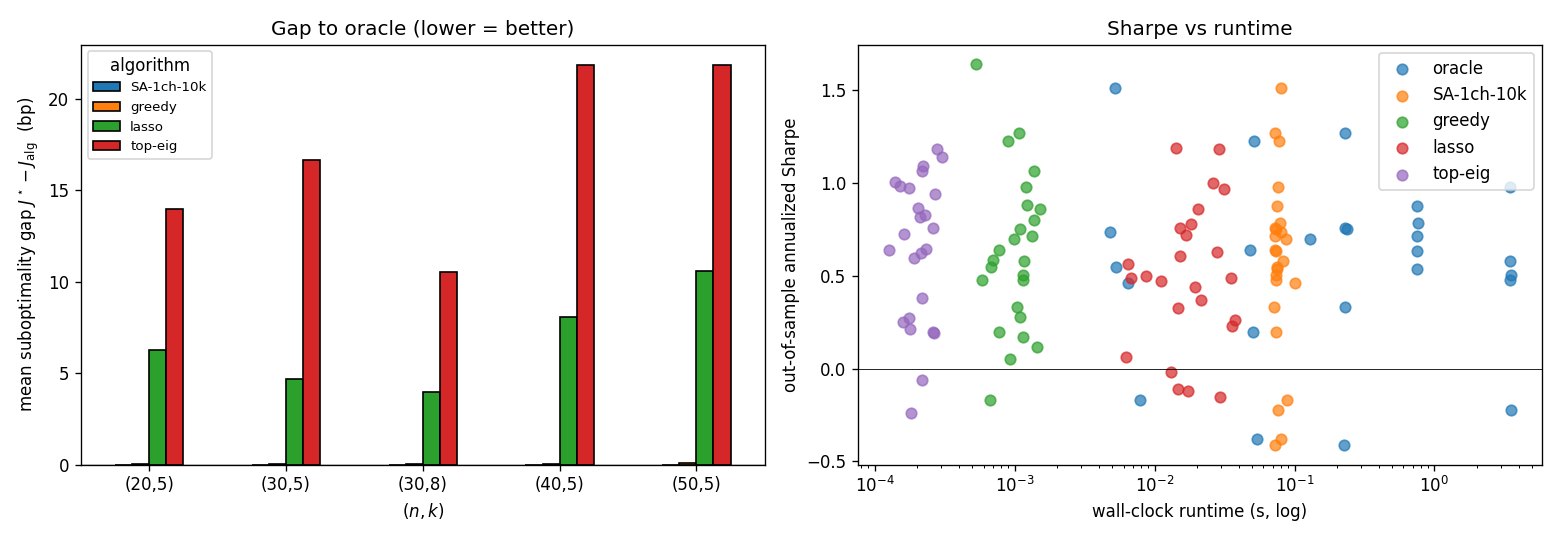
\includegraphics[width=\linewidth]{figs/oracle_vs_baselines.png}
  \subcaption{Oracle vs.\ baselines: optimality gap (bp) and oracle-match rate per $(n,k)$ cell.}\label{fig:oracle-baselines}
\end{minipage}\hfill
\begin{minipage}{0.36\textwidth}\centering
  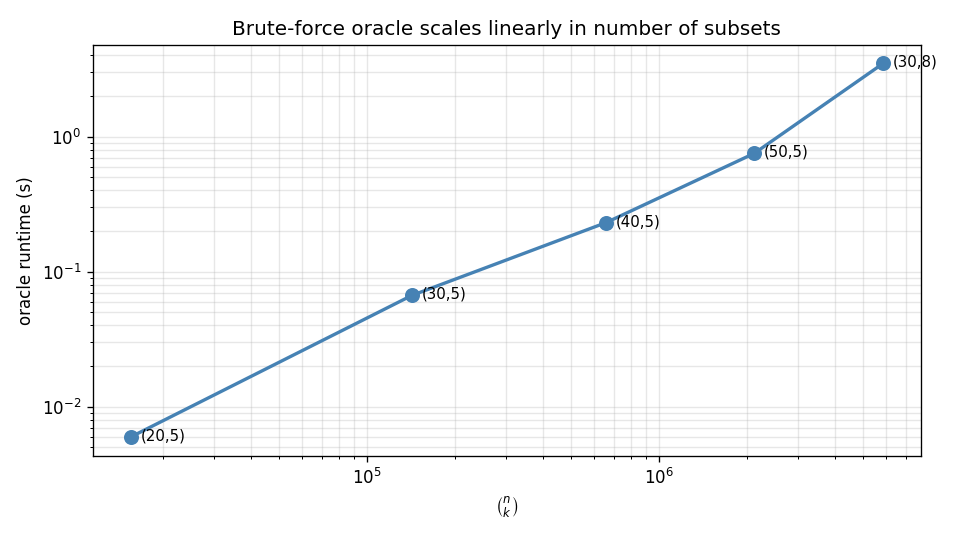
\includegraphics[width=\linewidth]{figs/oracle_runtime.png}
  \subcaption{Oracle runtime grows as $\binom{n}{k}$, reaching the $\sim\!10^7$-subset wall around $(50,5)$.}\label{fig:oracle-runtime}
\end{minipage}
\caption{Phase 2a benchmark on real S\&P 500 data. Simulated annealing matches the oracle on every cell within the brute-force range; LASSO is uniformly poor (RIP failure of \cref{fig:rip}), greedy is shockingly close, and top-eigenvector projection trails by $11$ to $22$\,bp.}\label{fig:phase2a}
\end{figure}

\subsection{Constrained Metropolis sampler and mixing diagnostics}\label{ssec:p2b}

The Boltzmann measure on the slice
\(
  \pi_\beta(\sigma) \;\propto\; \exp\bigl(\beta J(\sigma)\bigr),\quad \sigma\in\Omega_{n,k},
\)
is the natural object linking the empirical optimisation problem to the OGP machinery. We
implement a \emph{constrained Metropolis} chain on $\Omega_{n,k}$, viewed as a discrete-time
martingale-difference dynamics in the energy variable $J(\sigma_t)$ \cite{lec:mg}, with swap proposals
(remove one $i\in S$, add one $j\notin S$) and Metropolis acceptance
$\min\{1,\exp(\beta(J(S')-J(S)))\}$. With cached row-sums
$s_v := \sum_{j\in S}\hat\Sigma_{v,j}$, each swap evaluates in $O(1)$ amortised time
after $O(nk)$ initialisation; this gives the linear-in-$n$ samplers used throughout
Phases~3 and~4.

\paragraph{Validation against exact $\pi_\beta$.} On $(n,k)=(20,5)$ the slice has
$\binom{20}{5}=15{,}504$ states; we enumerate $\pi_\beta$ exactly and run the chain for
$3{,}000$ post-burn samples at $\beta\in\{0,50,200,10^3,5\!\times\!10^3\}$. The empirical
distribution matches the exact $\pi_\beta$ to within Monte-Carlo error (Kolmogorov-Smirnov
$p$-values $\ge 0.18$, with median $p=0.67$), confirming the chain's correctness.

\paragraph{Mixing-time blow-up: an empirical OGP precursor.} For each $(n,k,\beta)$ we run
$8$ independent chains for up to $1{,}500$ sweeps and record the median number of sweeps
to first hit the optimum $\sigma^\star$ (the \emph{hitting time} $\tau$). Results:

\begin{center}\small
\begin{tabular}{c|cccc}
$(n,k)\backslash\beta$ & $200$ & $1{,}000$ & $5{,}000$ & $20{,}000$\\\hline
$(20,5)$ & $\geq 1500$ & $\geq 1500$ & $769$ & $\mathbf{26}$\\
$(30,8)$ & $\geq 1500$ & $\geq 1500$ & $\geq 1500$ & $\mathbf{600}$\\
$(40,10)$ & $\geq 1500$ & $\geq 1500$ & $\geq 1500$ & $\geq 1500$\\
\end{tabular}
\end{center}

The $\tau \ge 1500$ entries are right-censored: the chain failed to reach $\sigma^\star$ in
the budget. The transition from $(20,5)$ (mixes in $26$ sweeps at $\beta=2\!\times\!10^4$) to
$(40,10)$ (does not mix even at $\beta=2\!\times\!10^4$) is a clear empirical
\emph{metastability transition}: the high-$\beta$ Boltzmann measure has multiple basins separated by
energy barriers that the chain cannot cross in polynomial time. This is exactly the
algorithmic signature of OGP, a \emph{topological} obstruction to dynamics rather than a
statistical one. The Phase~3 theory makes the obstruction quantitative.

\begin{figure}[ht]
\centering
\begin{minipage}{0.48\textwidth}\centering
  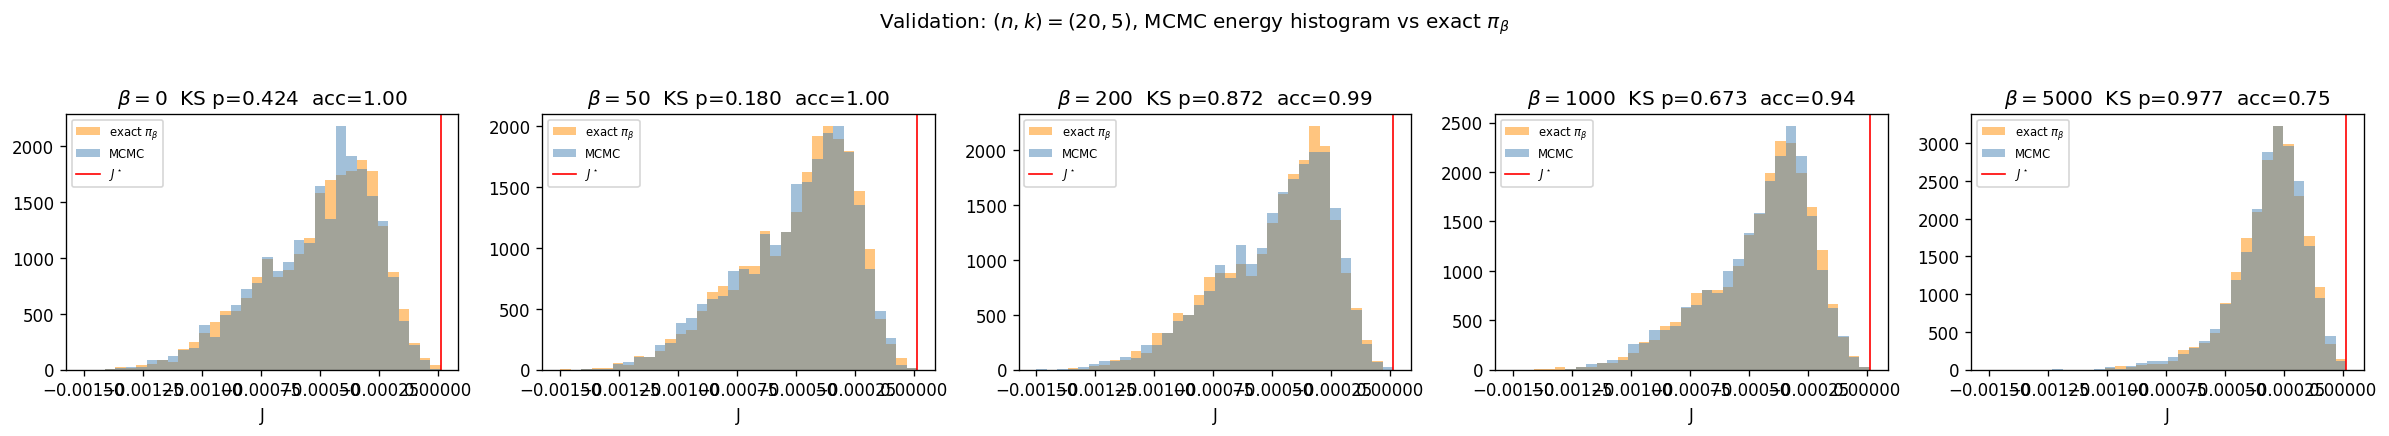
\includegraphics[width=\linewidth]{figs/mcmc_validation.png}
  \subcaption{Empirical CDF of $J(\sigma)$ from the chain (blue) vs.\ exact $\pi_\beta$ (red) on $(20,5)$ at five $\beta$. KS $p$-values $\ge 0.18$ confirm correctness.}\label{fig:mcmc-val}
\end{minipage}\hfill
\begin{minipage}{0.48\textwidth}\centering
  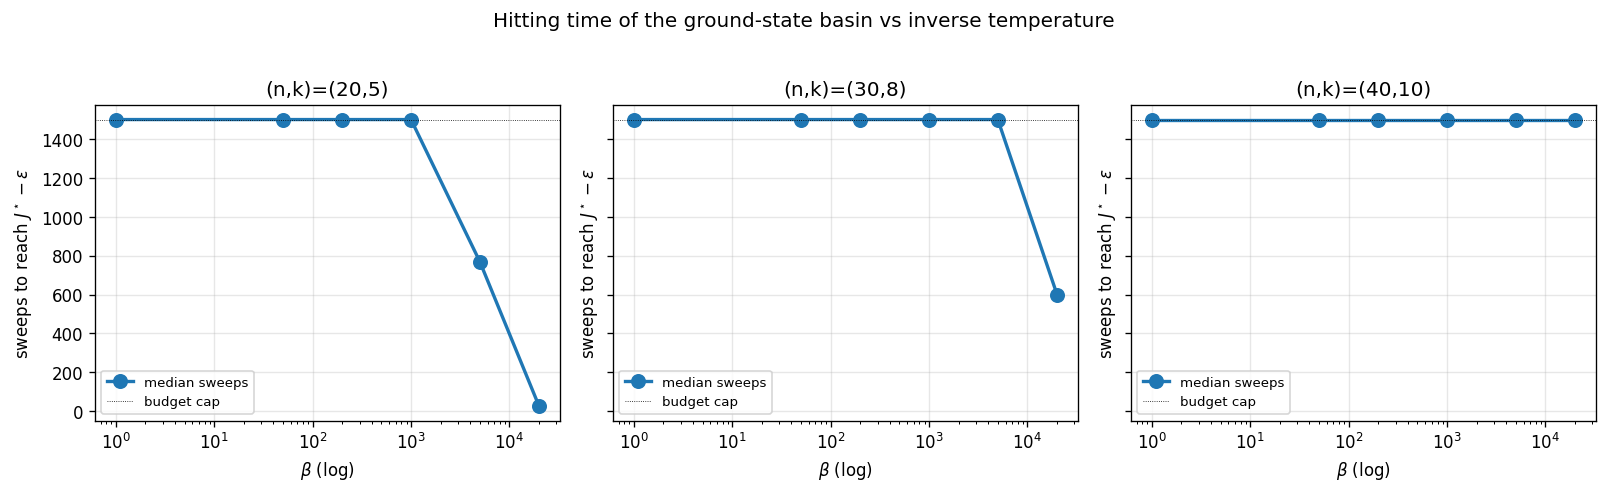
\includegraphics[width=\linewidth]{figs/mcmc_mixing.png}
  \subcaption{Hitting time $\tau$ of the optimum across $(n,k,\beta)$: rapid mixing on $(20,5)$, severe slowdown on $(40,10)$, the empirical OGP precursor.}\label{fig:mcmc-mix}
\end{minipage}
\caption{Constrained Metropolis sampler validation and mixing-time blow-up.}\label{fig:phase2b}
\end{figure}
